\documentclass[twoside]{article}
% \documentclass[journal]{IEEEtran}
% \documentclass[conference]{IEEEtran}
\usepackage[utf8]{inputenc}
\usepackage{a4wide} % Hierdoor worden de margins van de pagina kleiner
\usepackage{graphicx} % Voor grafische dingen zoals plaatjes, bijv. voor \includegraphics{herepathtofile}
\usepackage{enumerate} % Voor mooiere opsommingen
\setlength{\voffset}{-0.7in}
\setlength{\textheight}{650pt}
\setlength{\marginparwidth}{20pt}
\usepackage{xcolor}
\usepackage{caption}
\usepackage{hyperref}
\usepackage{adjustbox}
\usepackage{array}
\usepackage{booktabs}
\usepackage{multirow}
\usepackage{amssymb}
\usepackage{pifont}
\usepackage{scrextend}
\addtokomafont{labelinglabel}{\bf}
\usepackage{titlesec}
\usepackage{subcaption}

\usepackage{multicol}% http://ctan.org/pkg/multicols
\usepackage{amsmath}
\newcolumntype{R}[2]{%
    >{\adjustbox{angle=#1,lap=\width-(#2)}\bgroup}%
    l%
    <{\egroup}%
}
\newcommand*\rot{\multicolumn{1}{R{90}{1em}}}% no optional argument here, please!


\makeatletter
\def\mathcolor#1#{\@mathcolor{#1}}
\def\@mathcolor#1#2#3{%
  \protect\leavevmode
  \begingroup
    \color#1{#2}#3%
  \endgroup
}
\makeatother
\title{Machine Learning techniques for automatic ocular artifact correction in non-sleep resting state EEG:\\ practices and recommendations}
\author{Lisa Tostrams, Radboud University }
\date{July 2017}

\begin{document}

\maketitle

\tableofcontents

\section{Introduction}
\addcontentsline{toc}{subsection}{Problem description}
One of the methods used in the Center for Human Drug Research (CHDR) to asses the effect of a drug is resting state EEG. For the duration of a few minutes, cortical activity is measured in subjects who close and open their eyes. From the power spectrum of the measured signals some indications about the state of the central nervous system can be extracted. However, these measurements are often influenced by artifacts (e.g. eye and muscle movements). Currently, parts of the EEG recording are rejected when an artifact has been (sometimes manually) detected, which could mean a loss of relevant information. CHDR is interested in applying Machine Learning techniques to automatically detect and correct artifacts in EEG recordings. 


The aim of this report is to provide an overview of methods to analyze data from functional brain imaging (EEG) in the presence of (ocular) artifacts, using Machine Learning, filtering and pattern recognition. The purpose of these methods is to detect the presence of artifacts and recover the underlying EEG signal reflecting the true brain electrical activity. Besides providing an overview of methods, this report will recommend performance measurements and a modelling/experimental set up. %and establish the amount of data needed to asses and implement such methods.  

\subsection{Electroencephalography}
Electroencephalography (EEG) is a electrophysiological method to record electrical activity of the brain. The recording is non-invasive with electrodes placed on the scalp \cite{eegprinciples}, see figure \ref{fig:sensor} for placement. EEG measures voltage fluctuations resulting from ionic current within the neurons of the brain. The joint activity of millions of cortical neurons produce and electrical field that is sufficiently strong to be detected along the scalp. The amplitude of the EEG signal is related to the frequency of activity whether the excitation of the generating neurons is synchronized. The measured activity reveals oscillatory behaviour in specific frequency bands which are considered to be well-known EEG rhythms \cite{eegpatterns}. 

In measuring EEG, the interest typically lies in underlying neural potentials. The various wave forms of the EEG contain clinically valuable information, which make the methods for detection and quantification of characteristics to facilitate interpretation important \cite{eeg}. 

\begin{figure}
\centering

  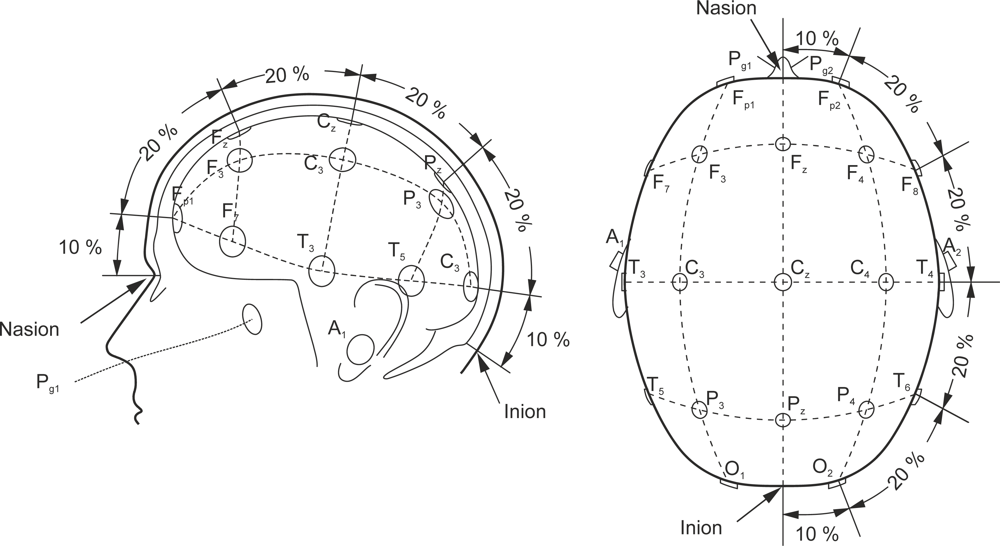
\includegraphics[width=.99\linewidth]{sensors-12-01211f1-1024}
  \caption{The electrodes for measuring EEG are placed over the scalp based on the International 10-20 system \cite{placement}. Using the nasion (located at the top of the nose) and the inion (located at the base of the skull) as reference, the skull is divided into planes. Electrode locations are determined by marking these planes at 10\% and 20\% intervals. The letters correspond to specific brain regions with, from front to back, Fp, F, C, P and O representing the fronto polar, frontal, central, parietal and occipital areas. The letter T represents the temporal area. A numbering system with odd numbers for the left hemisphere and even numbers for the right hemisphere is uses to differentiate between the sides. The subscript z on the central line stands for zero. Figure obtained from Nicolas-Alonso and Gomez-Gil (2012) \cite{BCI}.}
  

\label{fig:sensor}
\end{figure}

\subsubsection{Characteristics of EEG}
EEG can be described in terms of rhythmic activity and transients. The rhythmic activity is divided into bands by frequency, and activity within a band has been noted to have certain biological significance (see figure \ref{fig:patterns}.a) \cite{eegpatterns}. The rhythms have for example been noted to reflect different states of vigilance or aspects of cognitive processing. 

The amplitude of EEG varies from a few microvolts to approximately 100 $\mu$V. The amplitude can be well above this when corrupted by non-cerebral activity. The energy of the EEG signal is more concentrated in the lower range of the spectrum (see figure \ref{fig:freqency}). 
\begin{figure}
\centering

  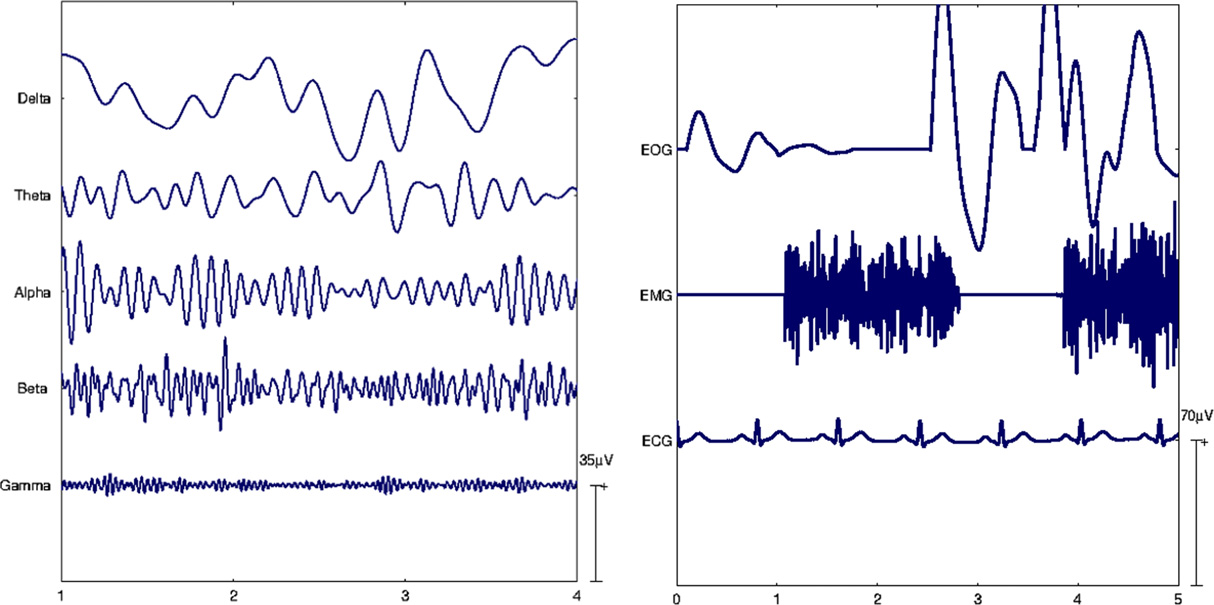
\includegraphics[width=.99\linewidth]{brainrythyms}
  \captionsetup{singlelinecheck = true, justification=raggedright }
    \caption*{ (a) Brain Rhythms \qquad \qquad\qquad \qquad  \qquad \qquad \qquad (b) Artifacts \qquad \qquad }

  \caption{(a) Examples of five normal brain patterns, from low to high frequencies, with usual amplitude levels. EEG patterns are characterized by their various frequency bands: delta (0.5-4 Hz), theta (4-7 Hz), alpha (8-13 Hz), beta (14-30 Hz) and gamma (30-100 Hz). (b) Examples of three kinds of artifacts: ocular, muscular and cardiac. Figure from \cite{eegguidelines}.}
  

\label{fig:patterns}
\end{figure}


\begin{figure}
\centering

  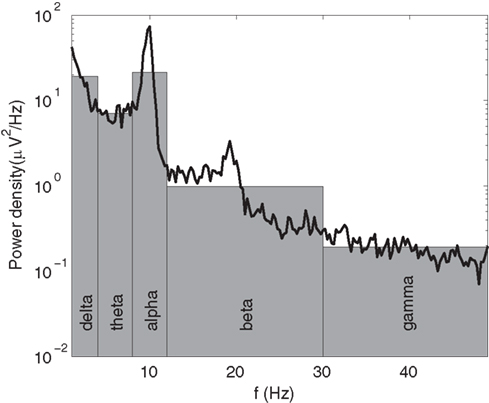
\includegraphics[width=.7\linewidth]{eegfrequency}
  \caption{Example of an EEG spectrum (black line) with an approximation of the different EEG pattern band powers, given by the areas of the grey bars. Figure from \cite{freqplaatje}.}
  

\label{fig:freqency}
\end{figure}


\subsection{Artifacts}
Signals detected by the EEG recording that did not originate from the cortex are considered artifacts. The EEG signal is often contaminated with various physiological factors other than cerebral activity \cite{eegguidelines}. Ocular movements and eye blinks are some of the most common types of biological artifacts (see figure \ref{fig:patterns}.b). The correction or rejection of artifacts is an important issue in EEG signal processing and a necessary component of most signal analysis. Manual inspection of EEG is a tedious task and automatic scoring is preferred \cite{nasa}. 

\subsubsection{Ocular artifacts}
The eye forms a electric dipole, where the cornea is positive and the retina is negative. Eye movements change the electrical field around the eye producing an electrical signal known as the electro-oculogram (EOG). 
The electrical activity produced by eye movement is usually strong enough to be recorded along with the EEG \cite{ocularartifacts}. As a result, EEG recordings are often significantly distorted. The eye-movement related voltages propagate to sites along the scalp with an inverse relation to the squared distance from the eyes. About 0.20 of the vertical eye-moment voltage reaches $F_z$, and this amount decreases posteriorly to about 0.05 at occipital sites. Blinking is another cause for contamination of the EEG, in a more abrupt manner than eye movement and with a higher amplitude. 

When the effect of ocular activity can be estimated, this signal can be removed from the EEG (EOG correction). 

\section{Performance Evaluation}
The greatest challenge for determining the relative efficiency and performance of each method is that in `real' data the uncorrupted desired signal is not known. The majority of techniques are evaluated with simulated data and thus the validity of conclusions depends on the fidelity of the used model \cite{eval}. Methods can first be assessed and compared to other methods by using simulations, but recorded EEG should be used as a final testbed for evaluating the true performance, reliability and reproducibility \cite{eegguidelines}. 


\subsection{Validation with simulated data}
One advantage of using simulated data $X^s(t)$ \begin{align} X^s(t) = B^s(t) + O^s(t) \end{align} where the superscript $^s$ denotes simulated signals and with $B^s(t)$ being the simulated clean signal and $O^s(t)$ being the simulated ocular artifact, as opposed to measured data $X(t)$, is that the quality of the a priori signal  and the signal after artifact removal $C^s(t)$ can be assessed through performance measures. For $M$ channels and $T$ measurements, each signal is a $MxT$ matrix. 


\begin{figure}
\centering

  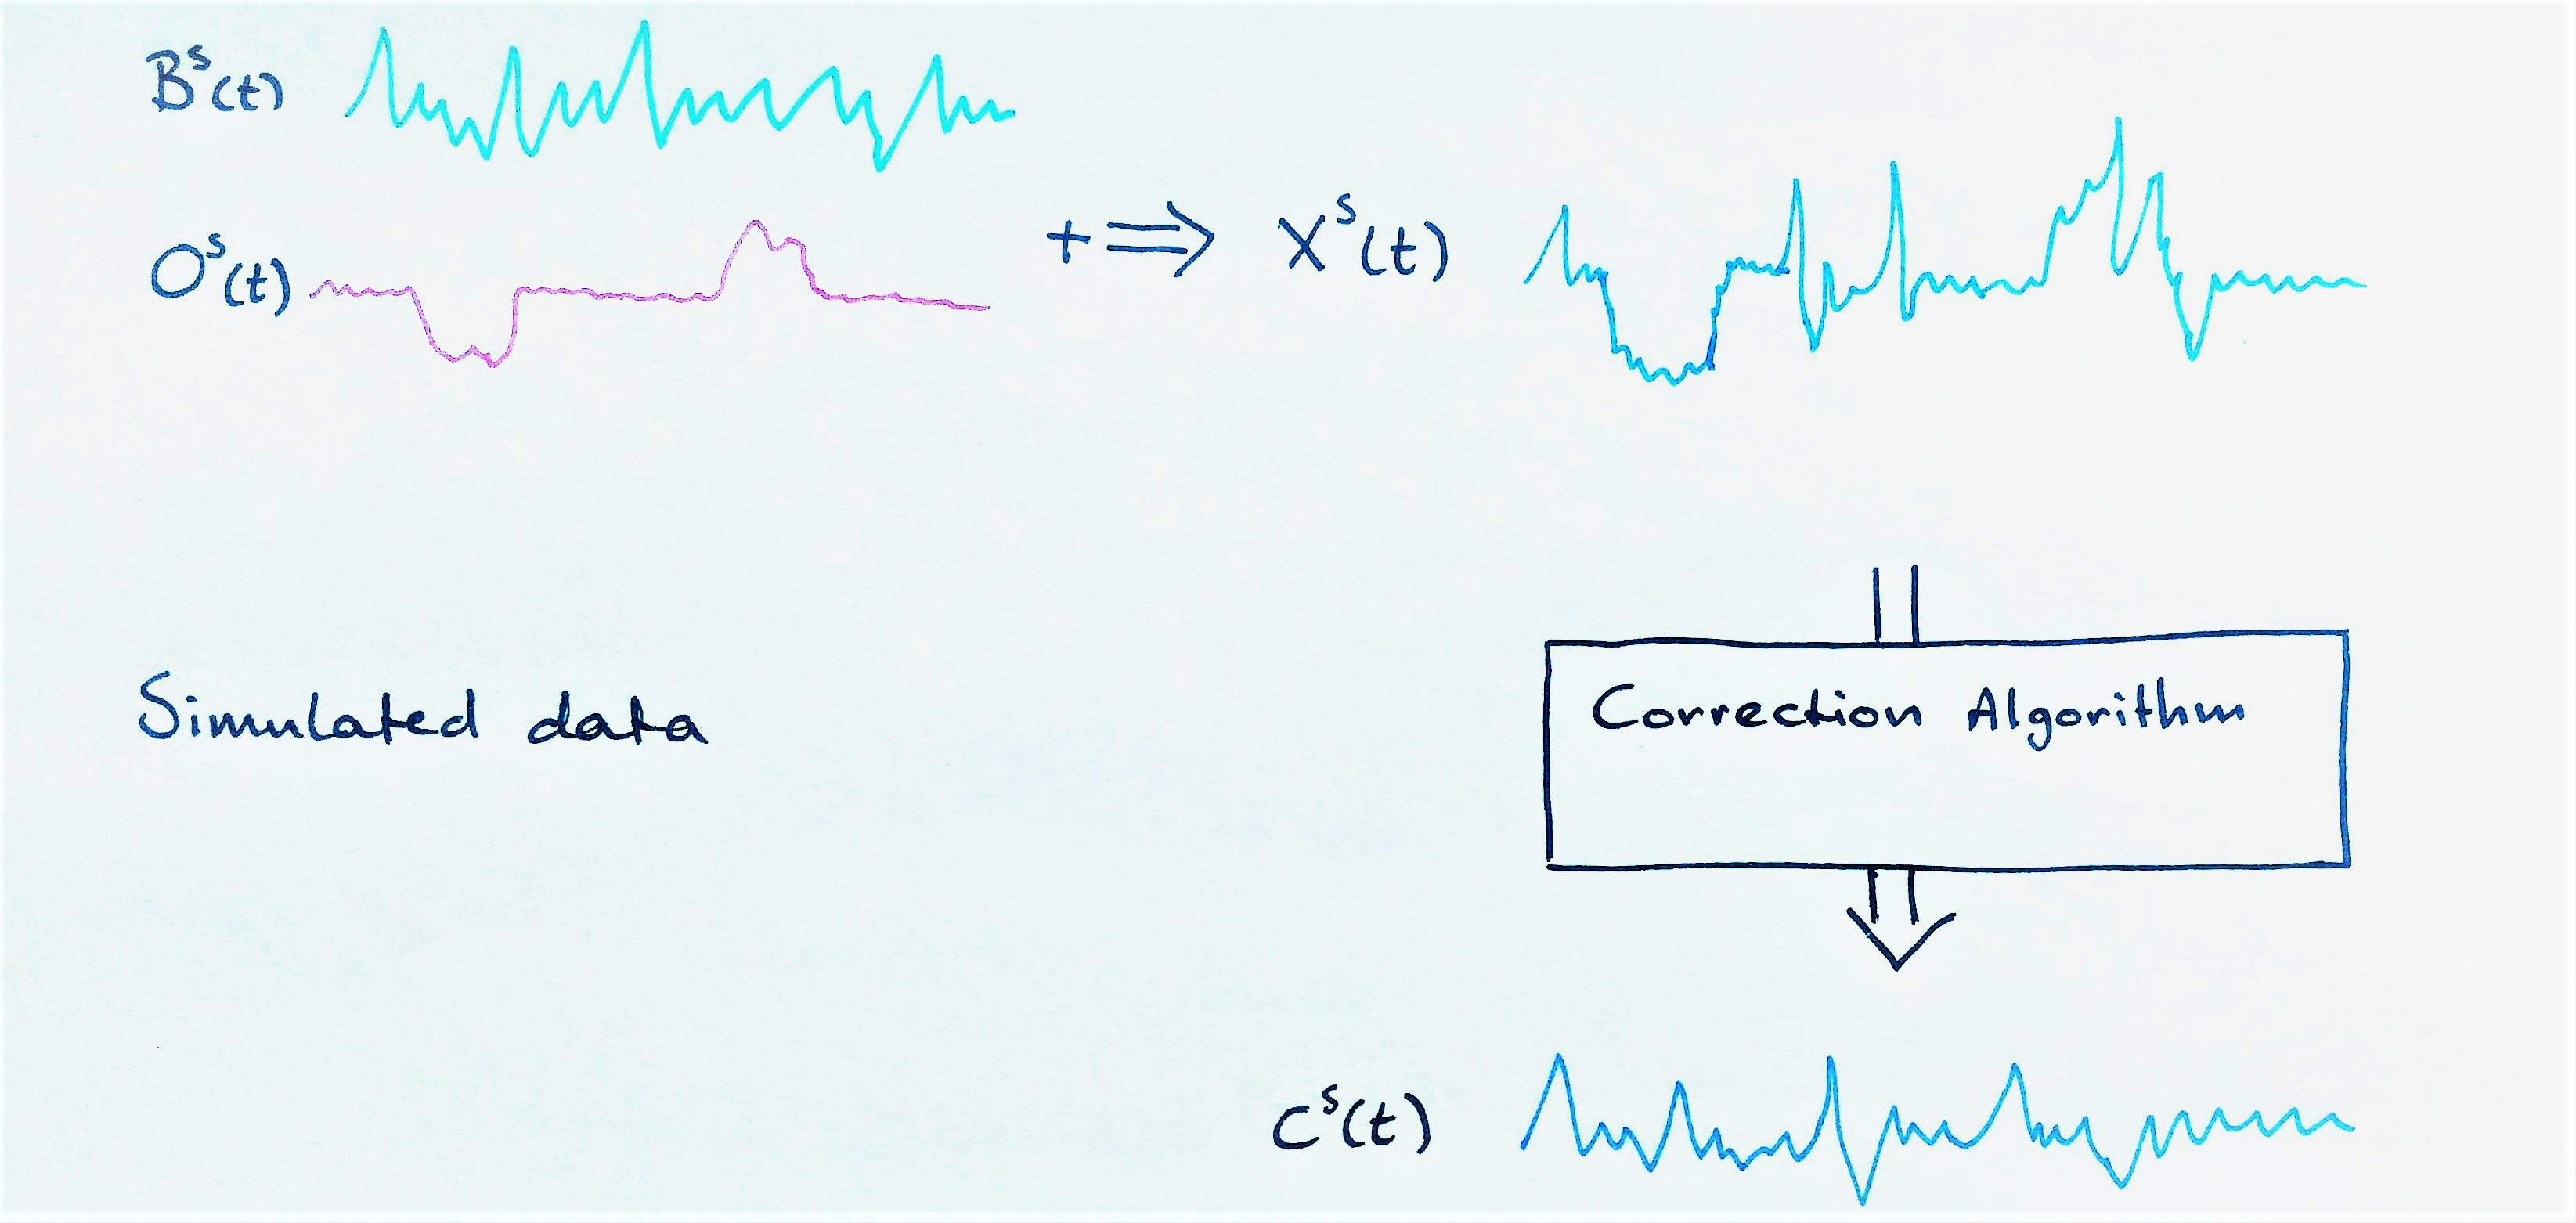
\includegraphics[width=.99\linewidth]{IMG_20170802_161247}
  \caption{\textcolor{red}{[FIX THIS IMAGE]} The simulated signal $X^s(t)$ is composed of the `true' signal $B^s(t)$ and the ocular artifact $O^s(t)$. The corrected signal of the simulated data $C^s(t)$ is obtained by applying an artifact correction algorithm. The improvement of the quality of the data after correction can be computed since the original artifact free signal $B^s(t)$ is known.}
  

\label{fig:simulations}
\end{figure}


\subsubsection{Percent correlation increase}
Correlation is used to describe the degree to which two variables have a linear relationship. The size of the correlation between two timeseries represents how much the two signals behave similarly. A correlation coefficient of near zero between two variables implies that they are linearly independent and a coefficient of near one implies a linear dependence (see figure \ref{fig:corr}). An increase of the correlation between the correlation of the artifact free signal $B^s(t)$ and the corrected signal $C^s(t)$ compared to the correlation of $B^s(t)$ with the corrupted signal $X^s(t)$ can be used as a measure for improvement. 

\begin{figure}
\centering

  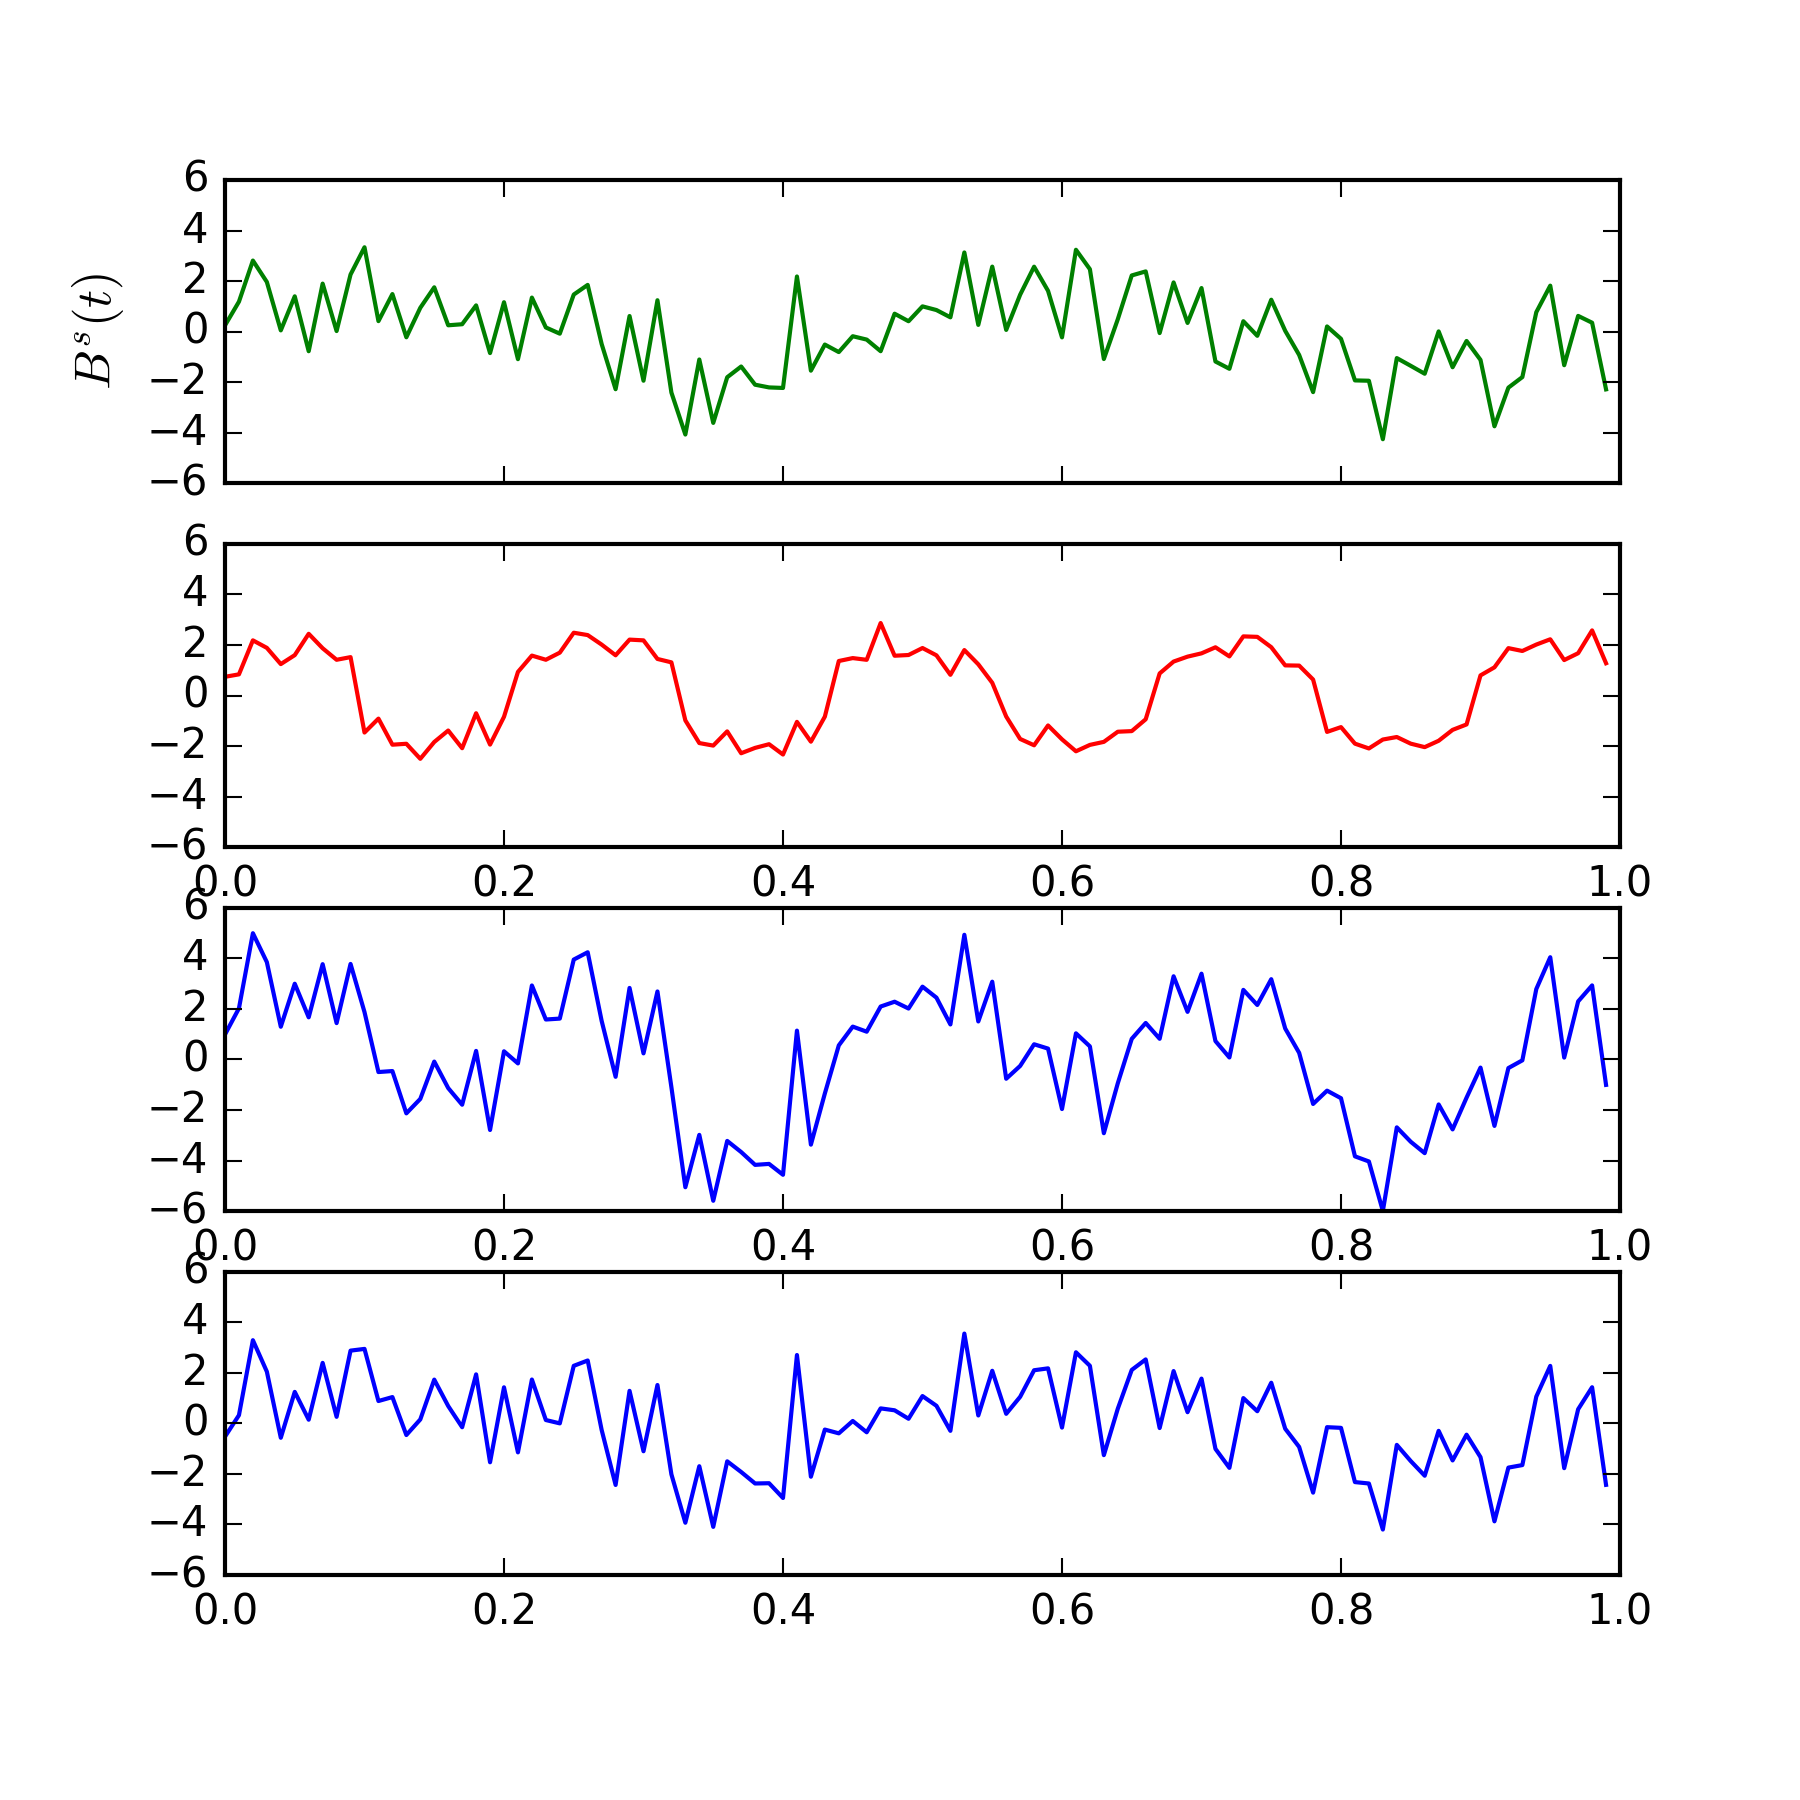
\includegraphics[width=.8\linewidth]{corr}
  \caption{Examples of two signals with a weak correlation (top) and a strong correlation (bottom). The correlation coefficient is 1.0 if there exists a perfect increasing linear relationship, -1.0 in the case of a perfect decreasing linear relationship, and some value in the open interval (-1.0, 1.0) in all other cases, indicating the degree of linear dependence between the variables. As the coefficient approaches zero there is less of a relationship and the variables are closer to being uncorrelated. The closer the coefficient is to either -1.0 or 1.0, the stronger the correlation between the variables.}
  

\label{fig:corr}
\end{figure}



The Pearson product-moment correlation coefficient $\rho$ of two timeseries $x(t),y(t)$ is defined as \begin{align} \rho = \frac{\frac{1}{T} \sum\limits_{t=1}^{T-1} (x(t) - \mu_x)(y(t) - \mu_y) }{\sigma_x \sigma_y}\end{align} with $\sigma_x$ and $\sigma_y$ being the standard deviations, and $\mu_x$ and $\mu_y$ the mean values of those timeseries.

The percentage increase in correlation after correction is calculated as \begin{align} \frac{\rho_a - \rho_c}{\rho_b - \rho_c} * 100\%\end{align} where $\rho_a$ is the correlation between $B^s(t)$ and $C^s(t)$ in the parts of the signal where artifacts occur, $\rho_c$ is the correlation between $B^s(t)$ and $X^s(t)$ in the same parts, and $\rho_b$ is the correlation of $B^s(t)$ and $X^s(t)$ in the parts of the signal with known clean data \cite{eval}.

\subsubsection{Signal to noise ratio}
The signal to noise ratio (SNR) is a measure of the relative amplitude of the artifact free signal $B^s(t)$ compared to the artifact  (the \textit{noise}) in any recording, see figure \ref{fig:snr}. The SNR is calculated per channel for both $X^s(t)$ and $C^s(t)$ with regards to the simulated artifact free signal $B^s(t)$  \cite{SNR}. For the a priori signal $X^s(t)$, the SNR is defined as \begin{align} SNR_X = \frac{\frac{1}{T} \sum^T_{t=1} B^s(t)^2 }{\frac{1}{T} \sum^T_{t=1} (X^s(t) - B^s(t) = O^s(t))^2} \end{align} Similarly, the SNR of the corrected signal is defined as \begin{align} SNR_C = \frac{\frac{1}{T} \sum^T_{t=1} B^s(t)^2 }{\frac{1}{T} \sum^T_{t=1} (C^s(t) - B^s(t))^2} \end{align}
The gain in SNR after correction can be calculated per electrode as \begin{align}\gamma = \frac{SNR_C}{SNR_X} \end{align} A gain of zero depicts no improvement after correction. The gain of a perfect correction approaches infinity. 
The overall score is obtained by averaging the $\gamma$-values of all M electrodes and converting to a decibel scale \begin{align}G = 20* \log_{10} \left [ \frac{1}{M} \sum^M_{m=1} \gamma_m \right ] \end{align}


\begin{figure}
\centering

  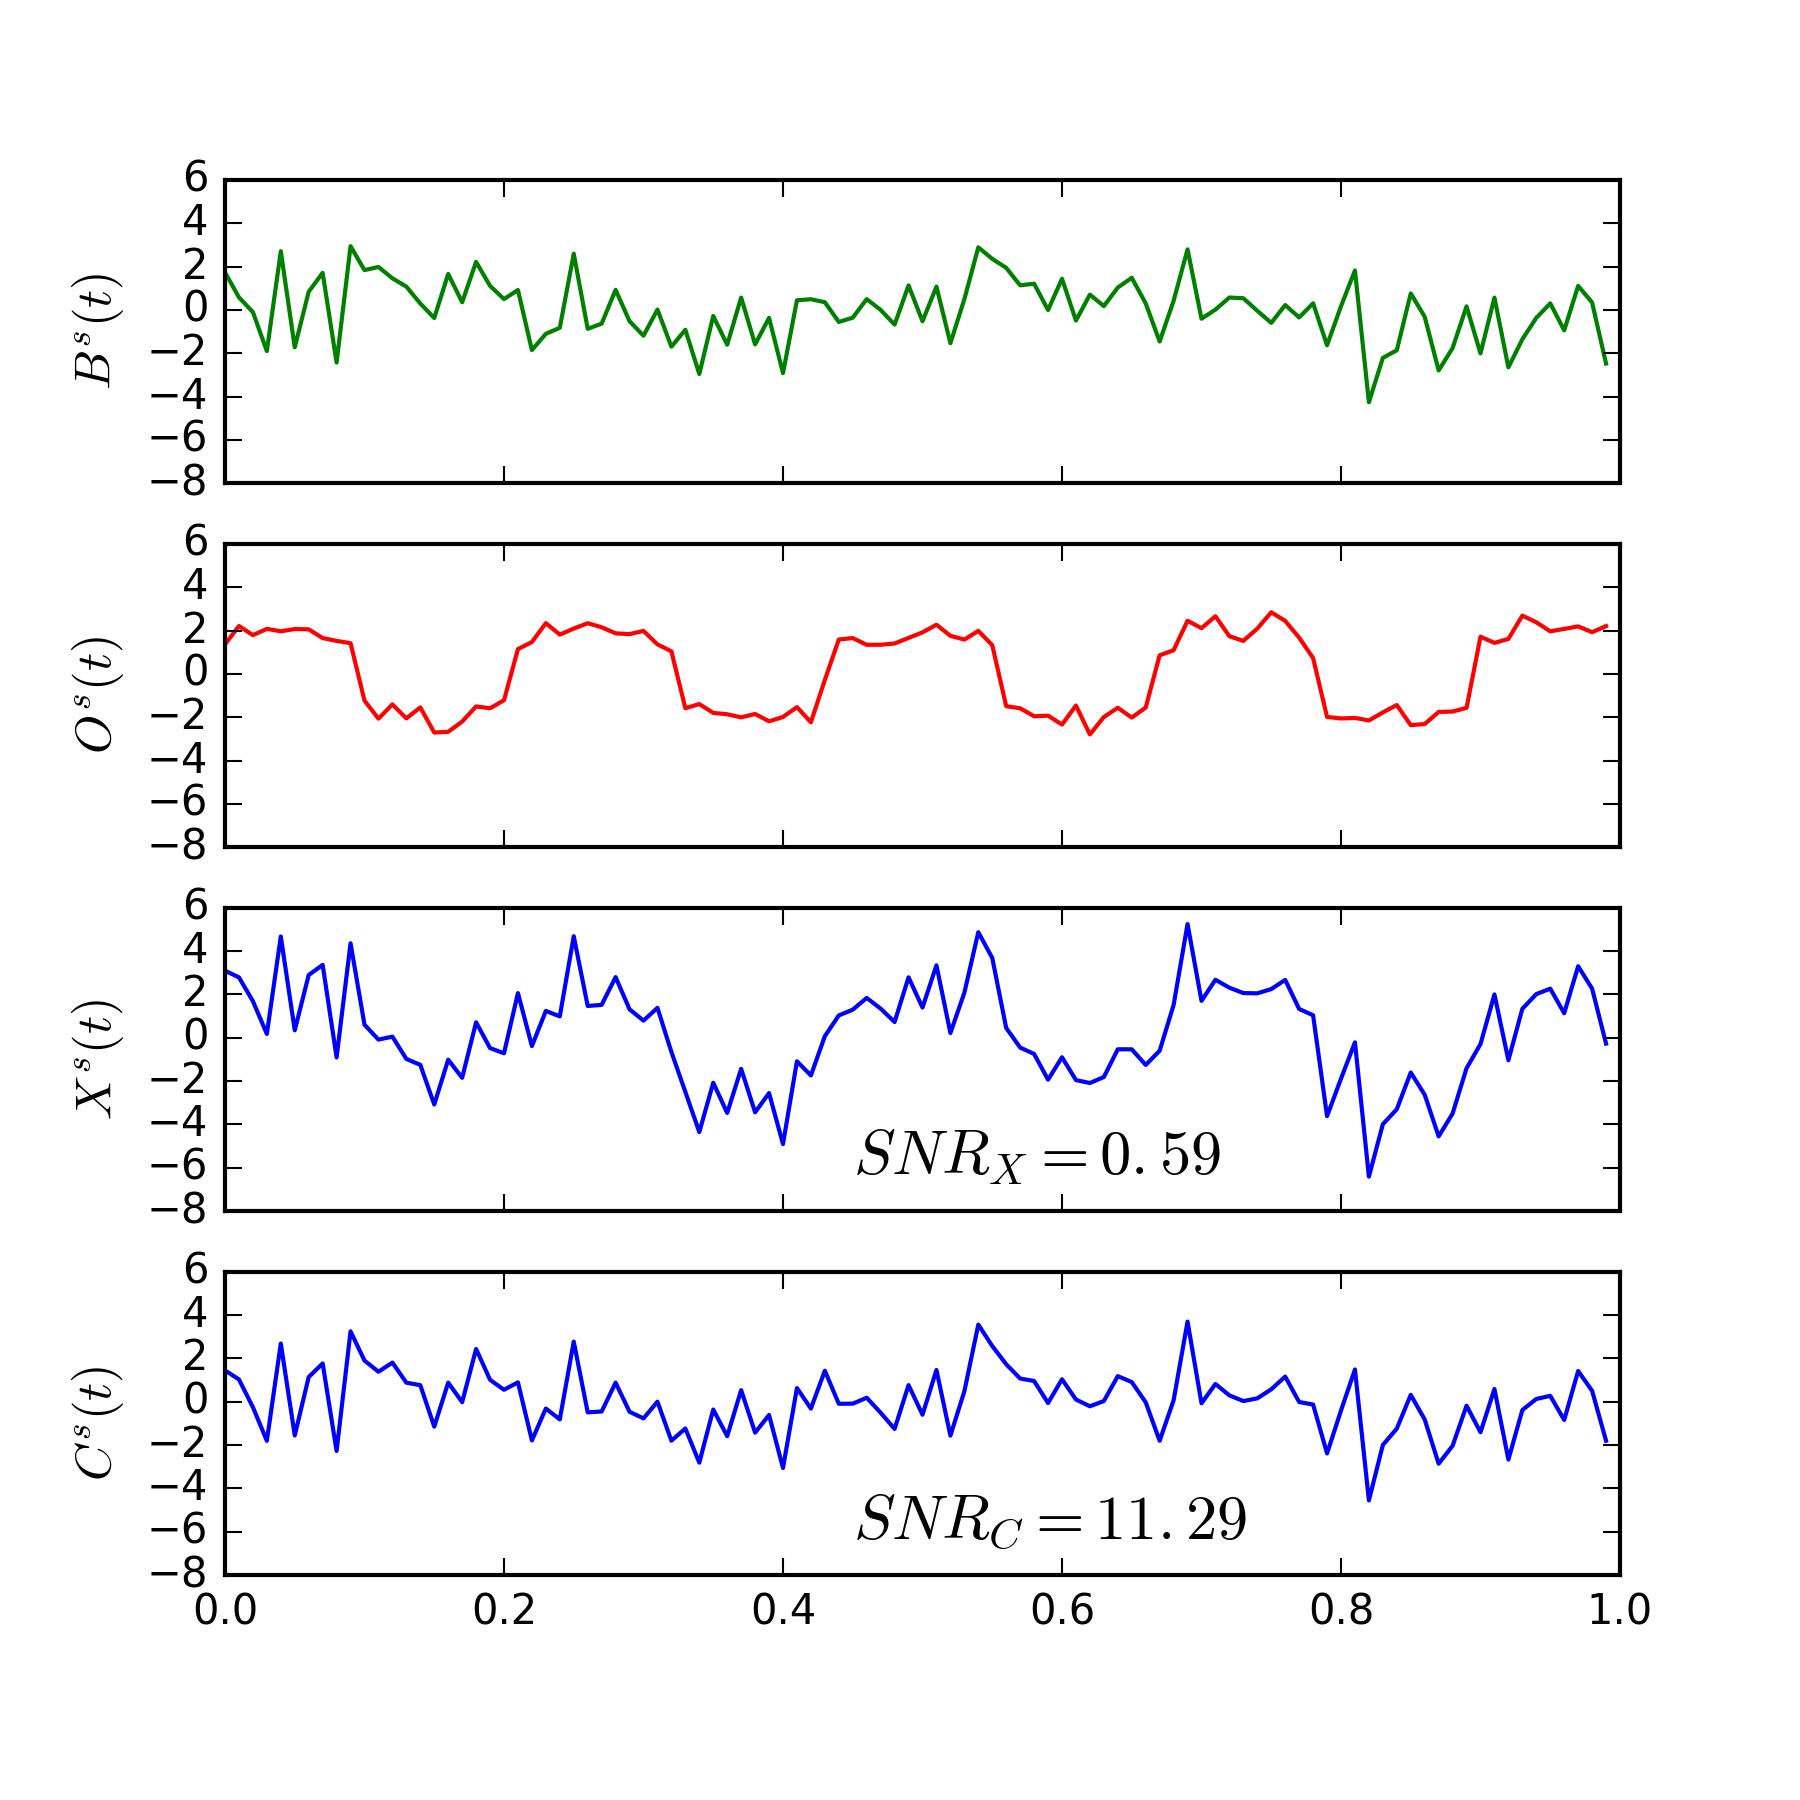
\includegraphics[width=.8\linewidth]{signals}
  \caption{Example of the SNR of some $X^s(t)$ and $C^s(t)$. For $X^s(t)$, the $SNR_X$ is effectively calculated as the relative size of $B^s(t)$ compared to the artifact $O^s(t)$. For the corrected signal, the $SNR_C$ reflects the relative size of $B^s(t)$ compared to any noise left in the signal after correction. In this case, the gain $\gamma = 14.58$ and the overall score $G = 20 *\log_{10}(14.58) = 23.27 dB$.  }
  

\label{fig:snr}
\end{figure}




\subsubsection{Normalized mean squared error}
The normalized mean squared error (NMSE) measures the deviation between the corrected signal $C^s(t)$ and the simulated clean signal $B^s(t)$ \cite{nmse}. A low NMSE implies that the corrected signal is more similar to the true artifact free signal. The NMSE is calculated for each channel as \begin{align}NMSE =  \left ( \frac{\sum^T_{t=1} (C^s(t) - B^s(t))^2}{\sum^T_{t=1} B^s(t)^2}\right ) \end{align}

\subsection{Validation with acquired data}
The validation of methods on acquired data $X(t)$ depends on a number of factors, of which the most important is the availability of reference channels. 

\subsubsection{Regression validation (with EOG channels)}
The electrooculogram (EOG) is measured from electrodes recording voltage changes close to the eyes, see figure \ref{fig:eogplaecment}. For vertical eye-movements, the vertical EOG (VEOG) is computed as the difference between voltages recorded above and below the eye. Horizontal eye-movements are measured as horizontal EOG (HEOG), the difference between voltages at the left and right outer canthi of the eyes. The radial component (REOG) of the eye-movement is measured by subtracting the average voltage at the eyes from the reference electrodes. 

Regression validation is based on the assumption that the EOG and EEG channels are relatively uncorrelated \cite{evaleog}. The correlation between the corrected data and the reference EOG channels is determined by employing least-squares linear regressions where corrected EEG is the criterion variable and the H- and VEOG channels the predictor variables. The resultant absolute unstandardized beta coefficients are testes for relations with repeated measures ANOVA. 

\begin{figure}
\centering

  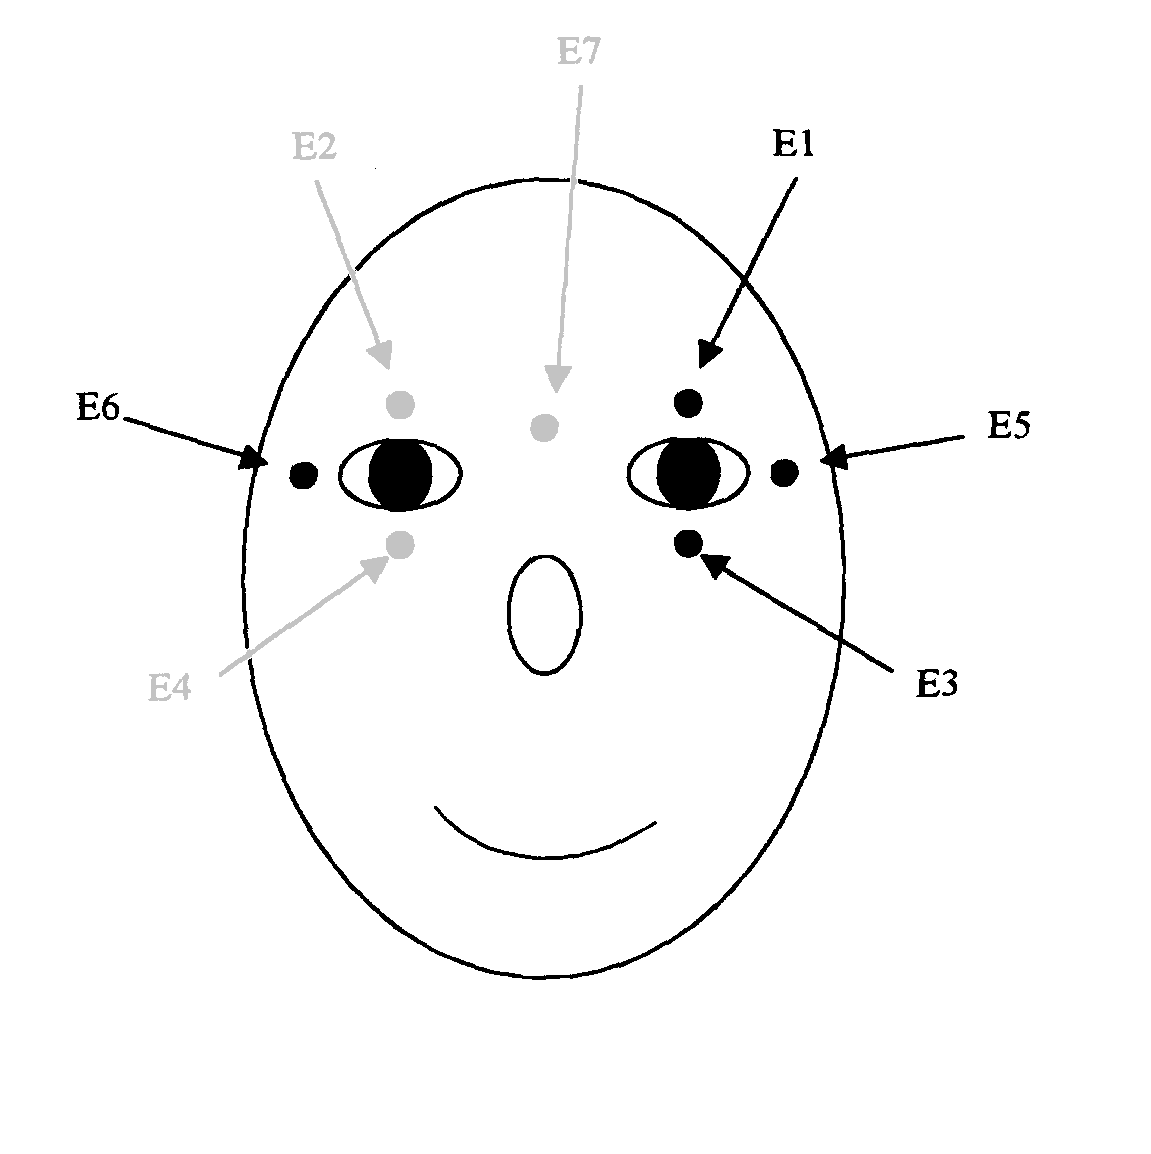
\includegraphics[width=.5\linewidth]{tilburgscheme}
  \caption{The electrode placement scheme used at the Tilburg symposium \cite{eogplacement}. For VEOG the difference between E1 and E3 is computed (E1-E3). For HEOG the difference between E5 and E6 is computed (E5-E6). REOG is computed as (E1+E3)/2. }
  

\label{fig:eogplaecment}
\end{figure}

\subsubsection{Simulate EEG from acquired data (with eye-tracker)}
By using eye-tracker data to simulate ocular movements, a signal of ocular movement related artifacts $O^s(t)$ can be simulated in EEG data \cite{SNR}. These artifacts are superimposed on simulated artifact free EEG signals $B^s(t)$. For subjects, the EEG is recorded at Cz position during a period of no eye movement. This can be verified with simultaneously recorded EOG and eye-tracker data. The resulting average frequency spectrum is used in the model to simulate EEG signals for the specific subject. Eye-tracker data is used to monitor the eye movements and determine the orientation of the source dipole (electrically active tissue).

\subsubsection{Intentionally corrupted and ground-truth channels (without reference channels)}
When there is full control of the EEG recording, two highly correlated signals can be produced: one that is a reference artifact free `ground-truth' signal, and one signal intentionally corrupted \cite{eval}. With these signals it is possible to apply artifact removal methods to the noisy EEG recording and compare the corrected signal to the ground-truth with methods proposed in section 3.1. 

\subsubsection{Quantitative evaluation of segments with ocular activity (without reference channels)}
Correction methods can be turned into detection methods by subtracting the corrected EEG signal from the raw EEG signal and thresholding the result. The resulting binary signal separates segments of the signal (or epoch) into computed zones with ocular artifacts and zones without \cite{evaleogdriving}, i.e. computed Ocular Artifact ($OA$) zones and non-OA zones ($\overline{OA}$) in figure \ref{fig:oa}.

\begin{figure}[h]
\centering

  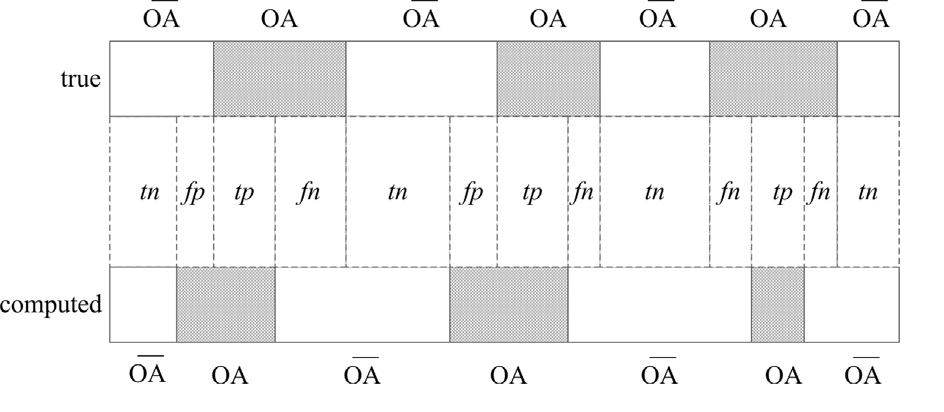
\includegraphics[width=.9\linewidth]{quantitative}
  \caption{The signal can be manually segmented in regions of Ocular Artifact ($OA$) zones and non-OA ($\overline{OA}$) zones to establish a ground truth. Comparing the true OA and non-OA zones to the zones computed by thresholding the correction defines the boundaries for the intervals of true positive ($tp$), true negative ($tn$), false positive ($fp$) and false negative ($fn$).  The length of these intervals define the customary $tp$, $tn$, $fp$ and $fn$ numbers required for computing sensitivity, specificity and the ROC curve. Figure from \cite{evaleogdriving}.}
  

\label{fig:oa}
\end{figure}

\begin{figure}[h]
\centering

  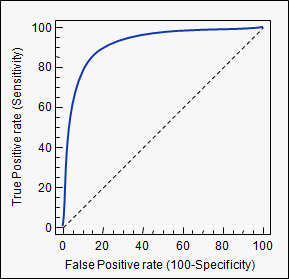
\includegraphics[width=.6\linewidth]{roc}
  \caption{An example of an ROC curve. First, the signals are segmented into zones of true and OA and non-OA (see figure \ref{fig:oa}). The computed OA and non-OA zones can be defined by thresholding the correction applied by some method. For each threshold, a pair of $tp$ and $fp$ rates can be computed. The thresholds range from the boundary that labels the entire signal as a non-OA zone (both $tp$ and $fp$ rates are 0) to the boundary that labels the entire signal as a OA zone (both $tp$ and $fp$ rates are 1, or a 100\%). Plotting all pairs of $tp$ and $fp$ rates results in a ROC curve. The dashed line on the diagonal depicts the curve for `random guessing' classification of zones, and has an Area Under the Curve (AUC) of 0.5 or 50\%. Any method whose curve is above the dashed line performs better than chance, and the more the curve approaches the optimal 100\% $tp$ rate vs 0\% $fp$ rate (upper left corner, classification results in an AUC closer to 1 or 100\%) the better the performance \cite{roc}.}
  

\label{fig:roc}
\end{figure}

To quantify detection performance, the ground truth can be defined by manually segmenting signals into true ocular artifact zones and true non-artifact zones, i.e. true OA ($OA$) zones and non-OA zones ($\overline{OA}$) in figure \ref{fig:oa}. The boundaries of the true and computed artifact zones define intervals that can be labeled true positive ($tp$), true negative ($tn$), false positive ($fp$) and false negative ($fn$), see figure \ref{fig:oa}. From these numbers, performance can be quantified by computing sensitivity (the proportion of artifacts that are detected) and specificity, defined as:

\begin{align}\textrm{sensitivity = \textit{tp} rate} = \frac{tp}{tp+fn}\end{align}


\begin{align}\textrm{specificity = 1 - \textit{fp} rate} = 1 - \frac{fp}{tn+fp} \end{align}

Another way to compare the performance is by plotting the receiver operating characteristics (ROC) curve, a technique for visualizing and selecting classifiers bases on their performance. An ROC curve depics the tradeoff between hit rates and false alarm rates of classifiers when different thresholds for classification are used ($tp$ vs $fp$ rates for different detection thresholds, see figure \ref{fig:roc}). ROC curves are especially important when considering domains with different classification error costs.

The results can be visually evaluated per epoch in the artifact affected zones, and quantitatively (area under ROC curve) for several epochs to compare performance between methods. 

\section{Methods}
Methods can be classified in 4 general groups: techniques using regression (EOG correction), filters, component analysis (blind source separation) and source decomposition. 
In general, each method can be augmented with thresholding for artifact detection, only correcting the signal during the affected intervals to save in computation time and to avoid perturbing the signal in time regions where the signal is not or less corrupted. 

\subsection{EOG correction \cite{ocularartifacts} \cite{eogcorrection} \cite{eogcorrection98}}
EOG correction generally refers to methods that assume the measured EEG $X(t)$ is a linear combination of the true signal $B(t)$ and ocular artifacts $O(t)$. The proportion of ocular activity present in each channel is calculated by regression. The correction is done by estimating and subtracting the regressed portion of the EOG reference wave forms from each EEG channel resulting in the corrected signal $C(t)$.  The use of two EOG channels (HEOG and VEOG) in the correction procedure provides a better correction than one, and so multiple regression is often used. EOG correction is known to over-correct due to bidirectional contamination of the EOG and EEG signals. Since the EOG is as much contaminated by the EEG as the other way around, a portion of the true EEG is subtracted from the signal as well. Another drawback is the need of propagation factors (i.e. how much of the ocular artifact reaches the electrodes from the front of the scalp to the back) to be constant and the assumption of linearity of the signals. 


\subsection{Filtering}
Filtering techniques try to adapt the filter in order to minimize the mean squared error between the corrected EEG signal $C(t)$ from the measured EEG $X(t)$, and the desired artifact free signal $B(t)$. The general advantages of filtering is that training data is not needed and that it is automated. 

\subsubsection{Adaptive filtering \cite{adaptivefilter} \cite{adaptivefilterocular} \cite{ieee} }
An adaptive filter is a system with a linear filter that has a transfer function controlled by variable parameters and a means to adjust those parameters according to an optimization algorithm. The adaption of filter parameters is based on minimizing the mean squared error between the filter output $C(t)$ and the desired signal $B(t)$. AF assumes that the sources of the true signal $B(t)$ and the artifact $O(t)$ are uncorrelated. The most common adaptation algorithms are Recursive Least Square (RLS) and Least Mean Square (LMS). RLS offers a higher convergence speed but LMS offers computational simplicity. The filter is controlled by a set of coefficients or weights $w(t)$. LMS is based on gradient search according to the equation $w(t+1) = w(t) + \mu e(t)X(t) $ where $w(t)$ is the weights vector at sample $t$, $X(t)$ is the input signal, $e(t)$ is the filters error and $\mu$ is the filters convergence factor.

To remove ocular artifacts with adaptive filtering, separately recorded vertical EOG and horizontal EOG signals are used as reference inputs. 


\subsubsection{Wiener filtering \cite{wiener} \cite{adaptivewiener} \cite{ieee} }
Wiener filtering produces a filter that minimizes the mean square error between the desired signal $B(s)$ and its estimate $C(t)$. The filter is calculated from the spectra of both the signal $\phi_{B}(\omega)$ and the noise $\phi_{O}(\omega)$, which are in turn estimated from the averages of spectra of the measured signals $X(t)$ or by obtaining pure eye blinking components with Independent Component Analysis. Therefore, Wiener filtering does not need a reference signal. The true signal $B(t)$ and the artifact $O(t)$ are assumed to be stationary linear stochastic processes with known spectral characteristics or known auto- and cross-correlations. The signal and the artifact are assumed to be uncorrelated. 


\subsubsection{Bayesian filtering \cite{bayesianfiltering} \cite{eegguidelines} \cite{ieee}}
Bayesian filtering refers to formulating the problem of estimating the state of a time-varying system that is indirectly observed in terms of Bayesian probability theory. The Bayesian filter produces an estimate $C(t)$ of the value of the true current state $B(t)$ for any $t$ from a probability distribution using all the available information contained in the observation history $X(0),...,X(t)$. The future states are assumed to be independent of previous states given the current state, and the estimate $C(t)$ for the current state requires formulating a joint probability distribution over all previous measurements. Therefore, Bayesian filtering is limited by its computational complexity. 

\begin{figure}[h]
\centering

  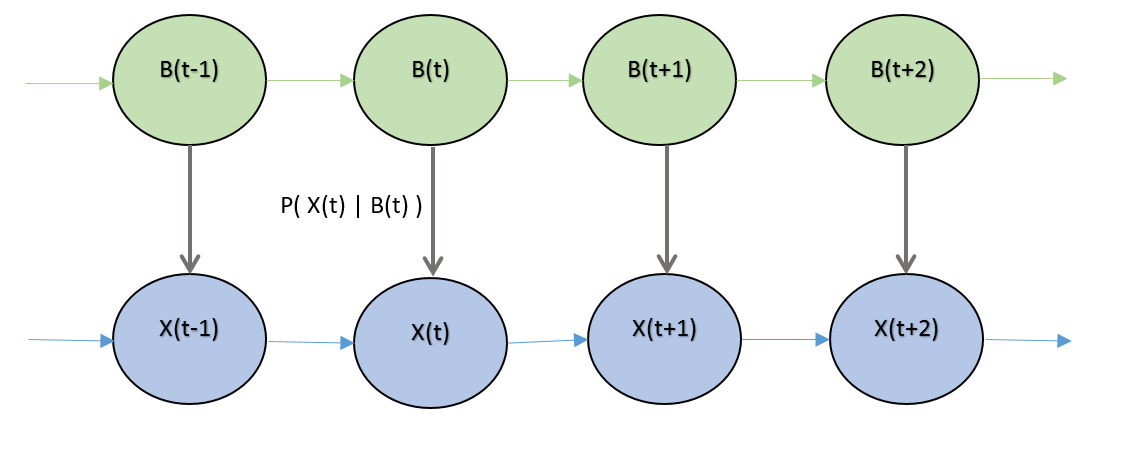
\includegraphics[width=.99\linewidth]{bayes}
  \caption{A Hidden Markov Model (HMM), a special case of a Bayesian network that represents sequences of values that are hidden and observations that are related to the hidden values by a (stationary) sensor model. The true signal $B(t)$ is unknown, but the observation (the measured EEG) $X(t)$ is related to $B(t)$ by the probability distribution $P(X(t) | B(t))$ known as the sensor model. Based on the observation history $X(0),...,X(t)$ the distribution of probabilities for the values of the current true state of the signal $B(t)$ can be computed. The estimate $C(t)$ of the current state is the value for $B(t)$ that is most likely based on the observation history.  }
  

\label{fig:bayes}
\end{figure}

For every observation $X(t)$ and true state $B(t)$ at any time $t$ the sensor model is defined by $P(X(t) | B(t))$, as depicted in figure \ref{fig:bayes}. These probabilities are computed from observed data and therefore a labeled training data set is needed. Using the Bayes rule, the distribution of probabilities for the current state $P(B(t) | X(0), .. , X(t))$ based on the observation history is computed. The corrected signal is then \begin{align}
C(t) = \textrm{arg max}_B P( B(t) | X(0), .. , X(t))
\end{align}
This computation step is exponentially complex with the number of observations, and therefore generally impossible to implement. Bayesian filtering assumes the process is Markov, meaning that knowledge of the current state contains all relevant information about the true process. Based on the same notions, the Kalman and particle filters approximate the Bayesian filter. 


\subsubsection{Kalman filtering \cite{kalman} \cite{adaptivewiener} \cite{kalmaneeg} \cite{ieee}}
The Kalman filter is a set of equations that provide a means to estimate the state of a process from a series of measurements in a way that minimizes the mean squared error. The algorithm for establishing the true signal $B(t)$ works in a two-step manner: in the prediction step, the filter produces an estimate of the current value $C(t)$ and its uncertainty. In the update step, the measurement $X(t)$ is used to update the estimate using a weighted average (the lower the uncertainty, the higher the weight). The Kalman filter needs a model for measurement noise and process noise variances to produce reliable predictions, but is only dependent on the current measurement and those models. If EOG is available, it can be used as an aid in the modeling of the signals. 


\subsubsection{Particle filtering \cite{ieee}}
Particle filtering uses Monte Carlo sampling to calculate a state transition model of the process. N samples are selected from a probability density function, and are weighted according to the amplitude of the probability density function at their sample point. A representative data set is needed to calculate the probability density functions. A large number of samples is needed to properly model the transition probabilities, with the optimal number of samples $N = \infty$ results in a Bayesian filter. The weights of new particles are determined using an update equation that uses the sensor model, and the estimated state $C(t)$ is the mean of the probability density function. Particle filtering depends less on the accuracy of process and sensor models than the Kalman filter, but may converge to the dominance of only a few particles resulting in improper corrections. 



\subsection{Blind Source Separation}
Blind source separation methods are used in signal processing to recover independent sources from signals that record a linear mixture of these sources. 

BSS uses the observations $X(t)$ to generate an unmixing matrix $W$ that determines an estimation of the original sources, including the artifact. With the original sources being the matrix representations of the true signal $B$ and the artifact $O$, $X$ is a linear combination $X = A\left[B+O\right]$ with mixing matrix $A$. Given the observation matrix $X$, the task is to estimate both the mixing matrix $A$ and the original sources $B+O$. Once the original sources of $X(t)$ are known, they can be selected and removed, and the signal is reconstructed without the artifacts to produce $C(t)$. 

BSS techniques generally require more electrodes than expected signal sources, and more time points than the square of the number of electrodes. Either the length of the recording or the sampling frequency can be increased to satisfy this requirement. BSS techniques fall in the class of unsupervised machine learning and do not need training data sets. In principle, the methods are not automatic but can be automated with reference channels. 


\subsubsection{Principal component analysis \cite{eegguidelines} \cite{tandm}}
Principal component analysis (PCA) is a statistical method that can be used to capture the variability of data in less attributes. PCA uses orthogonal transformation to represent the data in statistical uncorrelated variables called principal components. Reconstructing the data from a number of principal components that is smaller than the number of original variables causes the loss of a certain amount of variation in the data. PCA tends to identify the strongest patterns in the data. Since patterns caused by unlikely measurements are probably weaker than patterns caused by unlikely measurements, reduction of dimensionality can eliminate some of the measurement noise. The biggest problem with PCA for EEG applications is that the assumption of orthogonality between neural activity and typical physiological artifacts does not hold. 


\subsubsection{Independent component analysis \cite{eegguidelines} \cite{automatedica}}
Independent component analysis separates a multivariate signal into additive sub-components using only recorded information, by imposing statistical independence of the signal sources. This independence implies no spatial, temporal or time-frequency correlation between source signals. The ICA algorithms that exploit higher-order statistics (HOS-ICA) start by applying a orthogonal transformation (PCA), and then finding the linear transformation that results in the most independent estimated sources. ICA algorithms that apply second-order statistics are based on decorrelating the data in the time domain. Even when the assumption of independent sources does not exactly hold, ICA has been reported to be successful at removing artifacts. 

A drawback of ICA is the required intervention of a trained professional to manually identify the components related to artifacts. ICA can be combined with Bayesian classification to be automated, by computing the probability that an epoch represents EEG activity. Again, calculating the necessary probabilities for Bayesian learning is computationally intractable, but they can be estimated by using tree-augmented naive Bayesian networks that construct a maximum spanning tree based on feature dependencies.

When a reference signal is introduced, ICA (then ICA-R) can be automated as well. 


\subsubsection{Second order blind inference  \cite{SOBI}, \cite{SOBIautomated} \cite{SOBIreview}}
Second order blind inference (SOBI) uses decorrelation across several time points as its basic computational step. SOBI considers the relationship between components at different time lags and insists that these are decorrelated as much as possible. SOBI can be automated by identifying components that correlate with components from EOG channel recordings. Contrary to ICA, SOBI does not assume uncorrelated sources of the signals. 



\subsubsection{Canonical correlation analysis \cite{eegguidelines} \cite{ieee} \cite{cca}}
Canonical Correlation Analysis (CCA) measures the linear relation between two multidimensional random variables. CCA takes the source vector as the first multidimensional random variable and a temporally delayed version of the source vector as the second multi-dimensional random variable. By looking for uncorrelated components, CCA accounts for temporal correlations. Artifact removal can be introduced by setting the columns of the unmixing matrix that represent artifacts to zero during the reconstruction. CCA does not require independence of the sources. 



\subsection{Source decomposition methods}
Source decomposition methods can be applied to single channel recordings. They decompose each individual channel into basic wave forms that represent either the signal or the artifact. 

\subsubsection{Wavelets \cite{eegguidelines} \cite{ieee}}
The wavelet transform has been widely uses in the context of EEG denoising. The WT is unable to remove artifacts which overlap in the spectral domain. Good separation of the signal and noise depends on the wavelet basis and its similarity to the source signals, and requires manual selection or comparison to some experimentally-determined threshold. WT can be combined with ICA to overcome shortcomings of both these methods. A drawback is that it is not always true that a source signal can be represented by a single decomposition unit. 

\subsubsection{Empirical mode decomposition \cite{eegguidelines} \cite{ieee} \cite{emd}}
Empirical Mode Decomposition (EMD) is a technique for non-linear signal processing that aims at decomposing a signal into its basis functions called intrinsic mode functions (IMFs). Signals and artifacts can be represented by one or more IMF. These IMFs can then be used as inputs to an ICA algorithm. The technique is intended for non-linear signal processing, and it is known for its low robustness against noise. Manual selection of artifacts is required. 


\begin{table*} \centering
    \begin{tabular}{rl|*{10}{p{0.35cm}|}}
       % & & \multicolumn{10}{c}{Knowledge Areas} \\
        & \multicolumn{1}{r}{} &  \rot{No additional sensors} &  \rot{Automated} & \rot{No training data}  & \rot{No modelling} 
        & \rot{Computationally effective} & \rot{No manual checking of result} & \rot{Easy to implement} 
        & \rot{Does not assume linearity} & \rot{Does not assume independence} & \rot{Insensitive to sign inversion} \\
        \midrule
        \midrule
        \multirow{1}{*}{{Regression}}
        & EOG correction             & \textcolor{red}{ \textcolor{red}{ \textcolor{red}{\ding{53}}}} &  \textcolor{green}{\checkmark}  &  \textcolor{green}{\checkmark}  &   \textcolor{green}{\checkmark} &   \textcolor{green}{\checkmark} &  \textcolor{red}{ \textcolor{red}{\ding{53}}}  &   \textcolor{green}{\checkmark} &  \textcolor{red}{\ding{53}}    &  \textcolor{red}{\ding{53}}    &  \\
        \midrule
        \multirow{1}{*}{Filtering}
        & Adaptive filter               &  \textcolor{red}{\ding{53}} &   \textcolor{green}{\checkmark} &  \textcolor{green}{\checkmark}  &   \textcolor{green}{\checkmark} &   \textcolor{green}{\checkmark} &  \textcolor{red}{\ding{53}}  & ?   & ?  &  \textcolor{red}{\ding{53}}  &   \\
        & Wiener filter                 & \textcolor{green}{\checkmark}   & \textcolor{green}{\checkmark}   & \textcolor{green}{\checkmark}   &  \textcolor{red}{\ding{53}}  & \textcolor{green}{\checkmark}   & \textcolor{green}{\checkmark}   & \textcolor{green}{\checkmark}   & \textcolor{red}{\ding{53}} &  \textcolor{red}{\ding{53}}  &   \\
        & Bayesian filter               & \textcolor{green}{\checkmark}   & \textcolor{green}{\checkmark}   &   \textcolor{red}{\ding{53}} & \textcolor{green}{\checkmark}   &  \textcolor{red}{\ding{53}}  & \textcolor{green}{\checkmark}   &  \textcolor{red}{\ding{53}}  & \textcolor{green}{\checkmark}   & \textcolor{green}{\checkmark}   &   \\
        & - Kalman                      & $^1$ & \textcolor{green}{\checkmark}   & \textcolor{green}{\checkmark}   &   \textcolor{red}{\ding{53}}$^1$ & \textcolor{green}{\checkmark}   & \textcolor{green}{\checkmark}   & \textcolor{green}{\checkmark}   & \textcolor{green}{\checkmark}   &   \textcolor{red}{\ding{53}} &   \\
        & - Particle                    & \textcolor{green}{\checkmark}   & \textcolor{green}{\checkmark}   & \textcolor{green}{\checkmark}   &  \textcolor{red}{\ding{53}}  & \textcolor{red}{\ding{53}}  &  \textcolor{red}{\ding{53}}  & \textcolor{green}{\checkmark}   & \textcolor{green}{\checkmark}   & \textcolor{green}{\checkmark}   &   \\
        \midrule
        \multirow{1}{*}{BSS}
        & PCA                           & $^2$ &  \textcolor{red}{\ding{53}}$^2$ & \textcolor{green}{\checkmark}   & \textcolor{green}{\checkmark}   & \textcolor{green}{\checkmark}   &  \textcolor{red}{\ding{53}}  & \textcolor{green}{\checkmark}   &  \textcolor{red}{\ding{53}}  &   \textcolor{red}{\ding{53}} & \textcolor{green}{\checkmark}  \\
        & ICA                           & $^2$  &  \textcolor{red}{\ding{53}}$^2$  & \textcolor{green}{\checkmark}   & \textcolor{green}{\checkmark}   & \textcolor{green}{\checkmark}   & \textcolor{green}{\checkmark}   & \textcolor{green}{\checkmark}   &  \textcolor{red}{\ding{53}}$^3$  &  \textcolor{red}{\ding{53}}$^3$   &  \textcolor{green}{\checkmark}  \\
        & ICA+Bayes                     & \textcolor{green}{\checkmark}   & \textcolor{green}{\checkmark}   &  \textcolor{red}{\ding{53}}  & \textcolor{green}{\checkmark}   &  \textcolor{red}{\ding{53}}  & \textcolor{green}{\checkmark}   &   \textcolor{red}{\ding{53}} &  \textcolor{red}{\ding{53}}$^3$   &  \textcolor{red}{\ding{53}}$^3$   &  \textcolor{green}{\checkmark}  \\
        & SOBI                          &  \textcolor{red}{\ding{53}} & \textcolor{green}{\checkmark}   & \textcolor{green}{\checkmark}   & \textcolor{green}{\checkmark}   & \textcolor{green}{\checkmark}   & \textcolor{green}{\checkmark}   & \textcolor{green}{\checkmark}   & \textcolor{green}{\checkmark}   & \textcolor{green}{\checkmark}   &   \\
        & CCA                           & $^2$  &  \textcolor{red}{\ding{53}}$^2$  & \textcolor{green}{\checkmark}   & \textcolor{green}{\checkmark}   & \textcolor{green}{\checkmark}   & \textcolor{green}{\checkmark}   & \textcolor{green}{\checkmark}   & \textcolor{green}{\checkmark}   & \textcolor{green}{\checkmark}   &   \\
        \midrule
        \multirow{1}{*}{SD}
        & WT                            & \textcolor{green}{\checkmark}   &  \textcolor{red}{\ding{53}} & \textcolor{green}{\checkmark}   & \textcolor{green}{\checkmark}   & \textcolor{green}{\checkmark}   &  \textcolor{red}{\ding{53}}  &?   & ?  &   \textcolor{red}{\ding{53}} &   \\
        & EMD                           & \textcolor{green}{\checkmark}   &  \textcolor{red}{\ding{53}}  & \textcolor{green}{\checkmark}   & \textcolor{green}{\checkmark}   & \textcolor{green}{\checkmark}   &  \textcolor{red}{\ding{53}}  & ?   & \textcolor{green}{\checkmark}   & ?  &  \\
   \bottomrule
    \end{tabular}
    \captionsetup{singlelinecheck = false, justification=raggedleft }
    \caption*{$^1$ \small does not require models in the presence of EOG reference}
    \caption*{$^2$ \small can be automated in the presence of EOG reference}
    \caption*{$^3$ \small reported to work well even when assumptions are violated}
    \captionsetup{singlelinecheck = true, justification=justified}
    \caption{A comparison of the advantages and disadvantages of artifact correction methods}
    
\end{table*}

\subsection{Summary}


The use of different techniques depends greatly on the availability of reference channels and the assumptions that need to be satisfied. The goal of this report is to research automated methods for artifact correction, and some techniques depend on the presence of EOG channels to operate without manual intervention. See Table 1 for an overview of advantages and disadvantages for each considered method. The used criteria are: 
\begin{labeling}{Does not assume independence}
\item [No additional sensors] No additional sensors are needed for this method, e.g. EOG channels or eye trackers. While the addition of sensors is not necessarily a problem at CHDR, a simpler system could be preferred when the experiment has to be set up and broken down multiple times a day, since the sensors need to be placed at the exact same locations each time. 
\item [Automated] This method can be automated. Manual selection of artifact affected areas in EEG signals is a tedious task, and generally, an automated method is preferred. 
\item [No training data] The implementation of this method does not require training data. Methods that employ supervised machine learning methods require a labelled training data set, with both true signals and artifacts (and their relative occurrence) that resemble the data in the intended application. 

\item[No modelling] No a priori modelling of the artifact and or the true signal is needed. In methods that require models of the true signal and the artifact, performance greatly depends on the accuracy of the models and how the models can be generalized to multiple subjects. 
\item[Computationally effective] The method has either linear or polynomial time complexity, i.e. execution of the method is computationally feasible. 
\item[No manual checking of results] The corrections applied by the method do not need to be checked for over-correction, incorrect convergence of parameters, or perturbation in areas without artifacts. 
\item[Easy to implement] Method is easily implementable and runable on all CHDR computers, in Python 3.4 or higher using packages that do not need to be installed separately or can be installed using pyinstaller.  
\item[Does not assume linearity] The correction applied by this method does not assume that the measured EEG is a linear combination of the true signal and the artifacts. 
\item[Does not assume independence] The method does not assume that the sources of the EEG signal (e.g. EEG signals origination in different brain areas, artifacts) are statistically independent. 
\item[Insensitive to sign inversion] Inverting the sign of the artifact signal does not affect the performance of the method. 
\end{labeling}



\section{Recommendations}

\subsection{Validation}
Simulated signals provide a manageable means for the in depth testing and evaluation of methods. But reproducibility, as well as performance, should be concluded from applying methods on measured EEG signals \cite{eegguidelines}. A series of measurements under the same recording conditions should be obtained, producing equivalent EEG and artifact combinations. 

\subsubsection{Simulated data}
Methods can be compared to other methods by using simulations, and the result can be used as a guide for validation. To solve the problem of limited knowledge of the underlying artifact-free brain signal, a semi-simulated EEG data set can be used \cite{simulateddata}. In this data set, artifact-free EEG signals are manually contaminated with ocular artifacts. Since the data set contains the precontaminated EEG signals, the signal underlying the artifacts is known, and the performance of different methods can be objectively assessed with the validation methods described in section 3.1. By subtracting the true signals from the contaminated signals and thresholding the result, a binary time series with indications of artifacts can be obtained and used for training. 



\subsubsection{Acquired data}
Both with and without reference channels, to assess the performance and reproducibility of the methods a series of EEG data sets recorded under similar experimental conditions is needed. The choice of method and evaluation methods greatly depends on the application and the expected SNR of the EEG recordings. Therefore, the validation data should be similar to the data in the intended application. 

When EOG channels are available, regression validation is a good option \cite{evaleog}. The magnitude of the relation between the corrected data and the EOG channels is used to measure the proportion of artifacts left in the signal. This method requires manual selection of good and poor corrections of the regression technique.  

Another option that does not require EOG channels is quantitative evaluation of segments with ocular activity before and after correction. A labelled EEG data set is needed, with a binary time series indicating true intervals with and without artifacts. The correction of a method is measured and thresholded to obtain a computed series of intervals with and without thresholds. Performance of the classification of artifacts can be expressed in measures like ROC curve, sensitivity, and specificity. 

A combination of these two validation methods for acquired data is the best and most representative option to generalize the performance of methods to the intended applications.

%In a controlled setting, two electrodes are secured to the scalp of the subject using an electrode cap. The cap is manufactured using material that allows the movement of one electrode without disturbing the other. The two electrodes are placed in close proximity (20 mm) and two accelerometers are attached to ensure that the orientation of each accelerometer is kept consistent with respect to each other. Subjects are instructed to keep their eyes closed and to maintain a stationary head position throughout the experiment, limiting the number of artifacts. Each trial consists of 9 minutes with motion induced artifacts to Channel 2's electrode at 2 minute intervals. This artifact is induced by mechanically disturbing the electrode by pulling on the connecting lead \cite{SNR}.
\subsection{Methods}
One of the most efficient and simple filters that can be implemented is the Kalman filter. This filter is an approximation of the computationally intractable Bayesian filter, and solves the problem of computing exponentially growing joint probability distributions by making use of process and noise models that specify the likeliness of transitions of the true states and observations given the estimated true states. These models can be hard to estimate, however, the presence of an EOG reference channel can aid in modelling the process and noise signals.  

However, the literature on performance of the Kalman filter on EOG artifacts is limited. In contrast, BSS methods provide a more tested and reviewed class of techniques for the removal of EOG artifacts. ICA, SOBI and CCA can be automated with the use of reference channels, and have been proven to work well. Of the three, both SOBI and CCA require fewer assumptions on independence and non-Gaussian sources. 

These methods are from the class of unsupervised machine learning class and do not require training data. The Kalman filter needs calibration as the choice of expected measurement noise variation matters for the performance, but this can be estimated from reference channels. Either of the methods Kalman filter, SOBI and CCA would work well, with their performance depending on the expected artifacts that occur in the data and the validity of the assumptions that are required. 

A less practical, but nevertheless more interesting, option is the automation of ICA with Bayesian classification. In the reference paper \cite{automatedica}, the joint probabilities are computed from an maximum spanning tree optimized Bayesian network, greatly reducing the amount of computations from exponential complexity to linear. From an academic standpoint this is one of the more interesting methods, even though it would require a substantial training data set (200 recordings of labeled data) to learn feature dependencies. A training set can be generated from the simulated data as proposed in the next section. 


\bibliographystyle{plain}
\bibliography{lib} 

\end{document}





